\documentclass[12pt]{article}
\newcommand{\bottomMargin}{2cm}

\newcommand{\header}{
	ДИЗАЙН И АНАЛИЗ НА АЛГОРИТМИ - \\ ПРАКТИКУМ\\
	\vspace{0.1cm}
        Летен семестър, 2025 г., първо контролно\\
	\vspace{0.1cm}
}
\newcommand{\tl}{$0,1$ сек.}
\newcommand{\ml}{$256$ MB}

%---DOCUMENT MARGINS---
\usepackage{geometry} % Required for adjusting page dimensions and margins
\geometry{
	paper=a4paper, % Paper size, change to letterpaper for US letter size
	top=4cm, % Top margin
	bottom=\bottomMargin, % Bottom margin
	left=2cm, % Left margin
	right=2cm, % Right margin
	headheight=3cm, % Header height
	%footskip=1.5cm, % Space from the bottom margin to the baseline of the footer
	headsep=0.5cm, % Space from the top margin to the baseline of the header
	%showframe, % Uncomment to show how the type block is set on the page
}
\usepackage{cmap}

\usepackage[T2A]{fontenc}
\usepackage[bulgarian]{babel}
\usepackage{fontspec}
\setmainfont{Times New Roman}
\setsansfont{Times New Roman}
\setmonofont{Courier New}
\usepackage[math-style=TeX]{unicode-math}
\setmathfont{Latin Modern Math}

\usepackage[nobottomtitles*]{titlesec}
\titleformat
{\section} % command
{\normalfont\fontsize{14}{14}\sffamily\bfseries} % format
{} % label
{0pt} % sep
{} % before-code
\titlespacing{\section}{0pt}{0em}{0em}
\usepackage[dvipsnames]{xcolor}
\titleformat
{\subsection} % command
{\fontsize{14}{14}\itshape} % format
{} % label
{0pt} % sep
{} % before-code
[\vspace{-1em}{\color{BrickRed}\rule{0.2\textwidth}{0.2em}}\vspace{-0.7em}] % after-code
\titlespacing{\subsection}{0pt}{0.5em}{0em}

\setlength{\parskip}{0.5em}
\setlength{\parindent}{24pt}
\sloppy

\usepackage{fancyhdr}
\pagestyle{fancy}
\usepackage{setspace}
\fancyhead[L]{
	\begin{minipage}{\textwidth}
		
\includegraphics[width=2.8cm]{/structure/logo.png}
	\end{minipage}
}
\fancyhead[C]{
	\begin{minipage}{\textwidth}
		\centering\large{\bf{\header}}
		\vspace{-0.35cm}
	\end{minipage}
}
\usepackage{emoji}
\usepackage{makecell}
\usepackage{tabularray}
\AtBeginEnvironment{table}{\vspace{-0.2cm}}
\AtEndEnvironment{table}{\vspace{-0.2cm}}
\usepackage{float}
\fancyhead[R]{
	\begin{tabular}{r@{\hspace{0.2cm}}l}
		\emoji{hourglass-not-done}: & \tl \\ 
		\emoji{floppy-disk}: & \ml \\ 
	\end{tabular}%
}
\renewcommand{\headrulewidth}{0cm}
\fancyheadoffset[L]{1cm}
\fancyheadoffset[R]{1cm}

\raggedbottom

\usepackage{amsmath}
\usepackage{stmaryrd}

\usepackage{graphicx}
\graphicspath{{./}}
\usepackage[export]{adjustbox}
\usepackage{wrapfig}
\makeatletter
\patchcmd\WF@putfigmaybe{\lower\intextsep}{}{}{\fail}
\AddToHook{env/wrapfigure/begin}{\setlength{\intextsep}{0pt}}
\makeatother
\usepackage[inkscapearea=page,inkscapepath=./svg-inkscape]{svg}
\svgpath{{./}}

\usepackage{placeins}
\usepackage{caption}
\captionsetup[table]{
	skip=0.25em,font=it,
	singlelinecheck=false,justification=justified,indention=-24pt,
	margin={24pt, 0pt}
}

\usepackage{enumitem}
\setlist{itemsep=-0.4em,leftmargin=\parindent,topsep=-\parskip}
\newcommand{\tabitem}{\indent~~\llap{\textbullet}~~}

\usepackage{hyperref}
\hypersetup{
	colorlinks=true,
	citecolor=blue,
	linkcolor=blue,
	urlcolor=cyan,
}


\begin{document}
\section{Задача К3. Монети}
\begin{wrapfigure}{r}{0.30\textwidth}
	\begin{adjustbox}{width=0.30\textwidth}
		\includegraphics{2025/coins.jpg}
\begin{figure}
	    \centering
	    \includegraphics[width=0.5\linewidth]{coins.jpg}
	    \caption{Enter Caption}
	    \label{fig:enter-label}
	\end{figure}
		\end{adjustbox}
\end{wrapfigure}

След като се прибра от поредната командировка, професор Пикачу започна да разопакова багажа си и откри подарък от скъп приятел от Китай - книгоразделител. Тъй като професорът е неграмотен, единственото приложение на книгоразделителя, което му дойде на ум, беше да го използва като линийка за проектирането на новата си полица за монети. 

Полицата ще представлява множество от $m$ хоризонтално поставени на една височина дървени греди, всяка от които покрива интервала $[L_i, R_i]$. Никои две греди няма да се пресичат или припокриват. Професорът има $n$ монети в своята колекция, но за да ги представи в пълната си прелест, той иска всяка монета да бъде поставена в целочислена координата върху някоя греда, така че минималното разстояние $D$ между две различни монети да бъде колкото може по-голямо. 

Помогнете на професора като напишете програма \textbf{coins.cpp}, която по дадени числа $n$ - брой монети в колекцията, $m$ - брой греди, използвани за изграждането на полицата, и цели числа $L_i, R_i$, $1 \leq i \leq m$ - интервал, който покрива $i$-тата греда, намира максималното възможно $D$, което може да бъде постигнато. 

\subsection{Вход}

От първия ред на стандартния вход се въвеждат две цели положителни числа $n$ - броят
на монетите в колекцията и $m$ - броят греди, използвани за изграждането на полицата.
На всеки от следващите $m$ реда следват по две цели числа - $L_i, R_i$, съответстващи на координатите на левия и десния край на $i$-тата греда. Монета може да бъде поставена в край на интервал.

\subsection{Изход}

На стандартния изход програмата трябва да изведе едно число - максималното разстояние $D$, което може да бъде постигнато.


\subsection{Ограничения}

\vspace{0.1em}
\begin{itemize}
	\item $2 \leq  n \leq 10^5$
    \item $1 \leq  m \leq  10^5$ 
    \item $0 \leq L_i <= R_i \leq 10^{18}$ 
\end{itemize}

\subsection{Оценяване}
В тестове, носещи около $30\%$ от точките, $L_i, R_i \leq 10^5$.

\subsection{Пример}

\begin{table}[ht]
	\begin{tblr}{|l|l|X[j]|}
		\hline
		\textbf{Вход} & \textbf{Изход} & \textbf{Обяснение на примера}\\
		\hline
		\texttt
            {\makecell[lt]{5 3 \\ 9 9 \\ 4 7 \\ 0 2}} & \texttt{2} & Един начин да постигнем разстояние $D = 2$ е да разпределим монетите на координати $0, 2, 4, 6$ и $9$.\\
		\hline
	\end{tblr}
\end{table}
\end{document}
